\makeatletter
\def\input@path{{../../}}
\makeatother
\documentclass[../../main.tex]{subfiles}

\graphicspath{
	{../../img/}
	{../img/}
	{img/}
}

\begin{document}
	\section{Интегральная формула Коши}
	Далее нам понадобится:
	\begin{lemma}[об интеграле ФКП]
		Пусть $g(z)$ аналитична в многосвязной области $D \subset \C$ во всех 
		точках, кроме некоторого конечного числа $z_1, z_2, \dots z_n \in D$, 
		которые соответствуют некоторым удаленным областям из 
		$D,\ D_k \subset D,\ k = 
		\overline{1,n}$, так, чтобы $g(z)$ была полностью аналитичной в $D_0 = D 
		\setminus \bigcup \limits_{k=1}^{n} D_k$.
		
		Тогда, в случае непрерывности $g(z)$ на $l = \partial D$, имеем:
		\[\int \limits_{l} g(z) \ dz = \sum_{k=1}^{n} \ \oint \limits_{\partial D_k} 
		g(z) \ dz  \]
	\end{lemma}	
	\begin{proof}
	Для доказательства используем интегральную теорему Коши для многосвязных 
	областей. Используя полную границу
	\begin{center}
		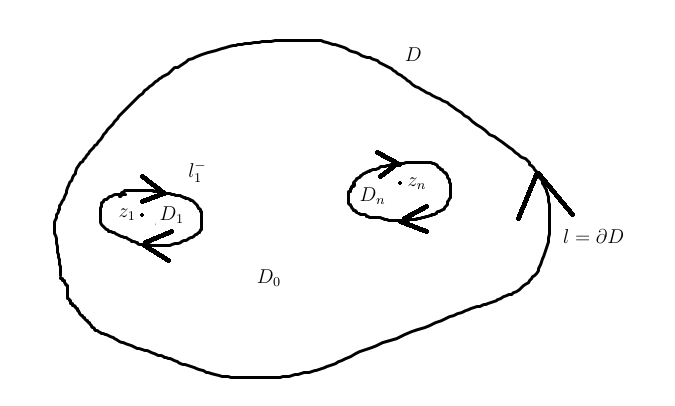
\includegraphics[width=0.7\linewidth]{lec32_1}
	\end{center}
	\[ l_0 = l \cup \left(\bigcup \limits_{k=1}^{n} l^{-}_{k}\right) \text{ на } 
	D_0 = D \setminus \bigcup 
	\limits_{k=1}^{n} D_k, \]
	где $g(z)$ аналитична в $D_0$, получаем, что:
	\[ \int \limits_{l_0} g(z) \ dz = 0. \]
	Тогда:
	\[ \int \limits_{l} g(z) \ dz + \sum^{n}_{k=1} \ \oint \limits_{ l_k} g(z) \ 
	dz = 0 \implies \int \limits_{l = \partial D} g(z) \ dz = - \sum_{k=1}^{n} \ 
	\oint \limits_{\partial l_k^{-} } g(z) \ dz = \sum_{k=1}^{n} \ \oint 
	\limits_{\partial l_k^{+} } g(z) \ dz. \qedhere \]
	\end{proof}	
\begin{theorem}[Интегральная формула Коши для ФКП]
	Пусть $f(z)$ аналитична в односвязной области $D \subset \C$, а $l_0 \subset 
	D$ \--- простой закмнутый контур, ограничивающий некоторый компакт $D_0 
	\subset D$, т.~е. $l_0 = \partial D_0$. Тогда $\forall z_0\in D_0 \implies$
	\begin{equation}
	\label{32:3}
	f(z_0) = \frac{1}{2\pi i} \ \oint \limits_{l_0} \frac{f(z)}{z-z_0} \ dz.
	\end{equation}
\end{theorem}
\begin{proof}
	Вначале заключим используемую точку $z_0 \in D_0$ в круг $K_R$ достаточно 
	малого радиуса $R>0$ с центром в $z_0$, целиком лежащим в $D_0$:
	\[ K_R = \left\lbrace z \in D_0 \ \big| \ |z-z_0| \le R\right\rbrace.  \]
	Пусть $l_R = \partial K_R = \left\lbrace t \in D_0 \ \big| \ |t-z_0| = R 
	\right\rbrace $. В силу предыдущей теоремы, имеем:
	\begin{equation}
	\label{32:4}
	\oint \limits_{l_0} \frac{f(z)}{z-z_0} \ dz = \oint \limits_{l_R} 
	\frac{f(t)}{t-z_0} \ dt.
	\end{equation}
	Рассмотрим область $G_0 = D_0 \setminus K_R$, получаем, что в \eqref{32:4} 
	подынтегральная функция
	\[ g(t) = \frac{f(t)}{t-z_0} \] аналитична в $G_0$.
	\begin{center}
		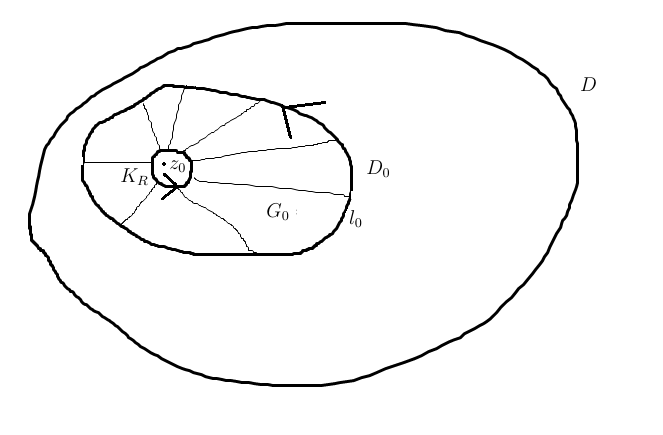
\includegraphics[width=0.7\linewidth]{lec32_2}
	\end{center}
	Значит,
	\[ \oint \limits_{\partial D_0^{+} \cup l_{R}^{-} }  g(t) \ dt = 0.   \]
	Используя важный пример
	\[  \oint \limits_{ l_{R}^{+} }  \frac{dz}{z-z_0} = 2 \pi i,    \]
	имеем:
	\[     \left| \frac{1}{2 \pi i} \oint \limits_{l_R} \frac{f(t)}{t-z_0} \ dt - 
	f(z_0)   \right| =  \left| \frac{1}{2 \pi i} \oint \limits_{l_R} 
	\frac{f(t)}{t-z_0} \ dt - \frac{f(z_0)}{2 \pi i} \oint \limits_{l_R} 
	\frac{dt}{t-z_0}   \right| = \left| \frac{1}{2 \pi i} \oint \limits_{l_R} 
	\frac{f(t) - f(z_0)}{t-z_0} \ dt  \right| = \]
	\[  \frac{1}{2 \pi }  \left| \oint \limits_{l_R} \frac{f(t) - f(z_0)}{t-z_0} 
	\ dt \right| \le  \frac{1}{2 \pi } \oint \limits_{l_R} \frac{ \left|  f(t) - 
	f(z_0) \right| }{ \left|  t-z_0   \right|   } \ \left| dt   \right| \le    \]
	\[  \le \left[ \begin{gathered}  
	f \ \text{равномерно непрерывна на} \ K_R, \text{тогда} \\
	\forall \eps >0 \quad \exists \delta = \delta_{\eps} > 0 \ : \forall t,z_0 
	\in K_R, |t-z_0| \le \delta  \implies
	|f(t) - f(z_0)| \le \eps \\
	r \le \delta
	\end{gathered}\right] \le   \]
	\[ \le \frac{1}{2\pi} \oint \limits_{l_R^{+}} \frac{\eps}{R} \ |dt| = 
	\frac{\eps}{2 \pi R } \oint \limits_{l_R^{+}} \ |dt| = \frac{\eps}{2 \pi R } 
	\cdot 2 \pi R = \eps     \]
	Т.~е. 
	\[  \forall \eps > 0 \quad \exists R \le \delta : \text{на} \ l_R = \partial 
	K_R \text{ такой, что}        \]
	\[ \left| \frac{1}{2 \pi i} \oint \limits_{l_0^+} \frac{f(t)}{t-z_0} \ dt - 
	f(z_0) \right| = \left| \frac{1}{2 \pi i} \oint \limits_{l_R^+} 
	\frac{f(t)}{t-z_0} \ dt - f(z_0) \right| \le \eps.    \]
	Отсюда, в силу того,  что $l_0$~--- фиксированный, а $\forall \eps > 0$, 
	получаем \eqref{32:3}.
\end{proof}	
\begin{remarks}
	\;
	
	\begin{enumerate}
		\item Если $f(z)$ аналитична в $D$ и непрерывна на $D$, то тогда формула 
		\eqref{32:3} верна и для $l_0 = \partial D$.
		\item Если $z_0 \notin D$, то $g(z) = \frac{f(z)}{z-z_0}$ \--- аналитична в 
		$D$, и значит:
		\[  \oint \limits_{l_0} \frac{f(z)}{z-z_0} \ dz = 0  \]
		\item Для $z_0 \in D$, используемой в \eqref{32:3}, формулу можно переписать 
		в виде:
		\begin{equation}
		\label{32:5}
		\oint \limits_{l_0^+} \frac{f(z)}{z-z_0} \ dz = 2 \pi i f(z_0)
		\end{equation}
		что можно использовать на практике для вычисления интеграла ФКП.
	\end{enumerate}
\end{remarks}	
\begin{examples}
	\begin{enumerate}
		\item 
		\[ I = \oint \limits_{|z| = \pi} \frac{z \ dz}{z^2 + 2z - 3}  \]
		\begin{center}
		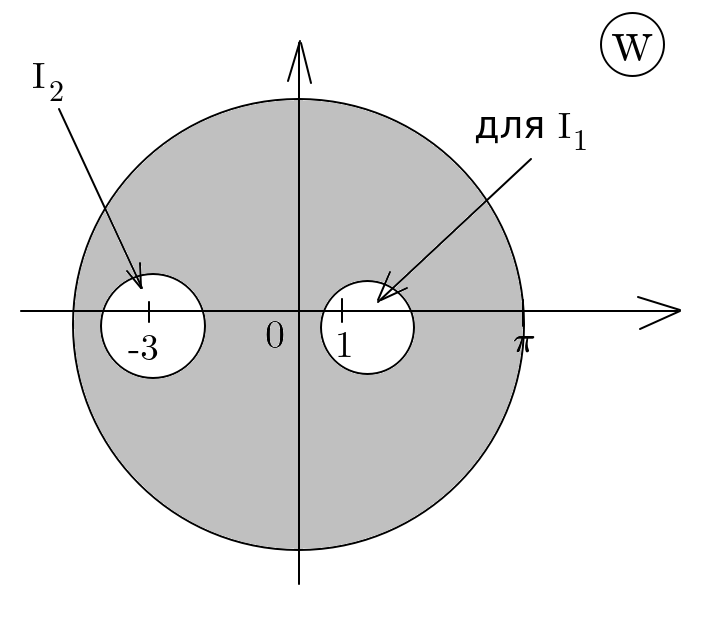
\includegraphics[width=0.42\textwidth]{lec32_3}
		\end{center}
		Здесь у подынтегральной функции $g(z) = \frac{z}{z^2 + 2z - 3}$, в области, 
		ограниченной контуром $|z| = \pi$, имеется две особенности $z_1 = -3,\ z_2 = 
		1$. В остальных точках $g(z)$ аналитична.
		\[  g(z) = \frac{A}{z-1} + \frac{B}{z+3} = \dots = \frac{1}{4(z-1)} + 
		\frac{3}{4(z+3)}  \]
		Отсюда следует, что:
		\[ I = I_1 + I_2.  \]
			\paragraph{Способ 1:}
			\begin{itemize}
				\item[а)]
				$\displaystyle I_1 = \frac{1}{4} \oint \limits_{|z-1| = 1} \frac{dz}{z-1} 
				= \left[ 
				\begin{gathered} f(z) \equiv 1 \\
				z_0 = 1 
				\end{gathered} \right] = \frac{1}{4} \cdot 2 \pi i = \frac{\pi i }{2}    .$
				\item[б)]  
				$\displaystyle  I_2 = \frac{3}{4} \oint \limits_{|z+3| = \frac{1}{10}} 
				\frac{dz}{z+3} = 
				\left[ \begin{gathered} f(z) \equiv 1 \\
				z_0 = 3 
				\end{gathered} \right] = \frac{3}{4} \cdot 2 \pi i = \frac{3 \pi i }{2}    
				.$
			\end{itemize}
			Получаем $ I = 2 \pi i $.
			\paragraph{Способ 2:}
			\[I = I_1 + I_2\]
			\[ I_1 = \oint \limits_{|z-1| = 1} 
			\frac{\frac{z}{z+3}}{z-1} \ dz = 2 \pi i \cdot \frac{z}{z+3} \bigg|_{z=1} = 
			\frac{\pi i}{2} \]
			\[ I_2 = \oint \limits_{|z+3| = \frac{1}{10}} \frac{\frac{z}{z-1}}{z+3} \ 
			dz = 2 \pi i \cdot \frac{z}{z-1} \bigg|_{z=-3} = \frac{3 \pi i}{2}  
			 \]
			 Откуда
			$ I = 2 \pi i. $
	\item \[ I = \oint \limits_{|z|=5,1} \frac{dz}{\sin{\pi z}} \]
	\begin{center}
		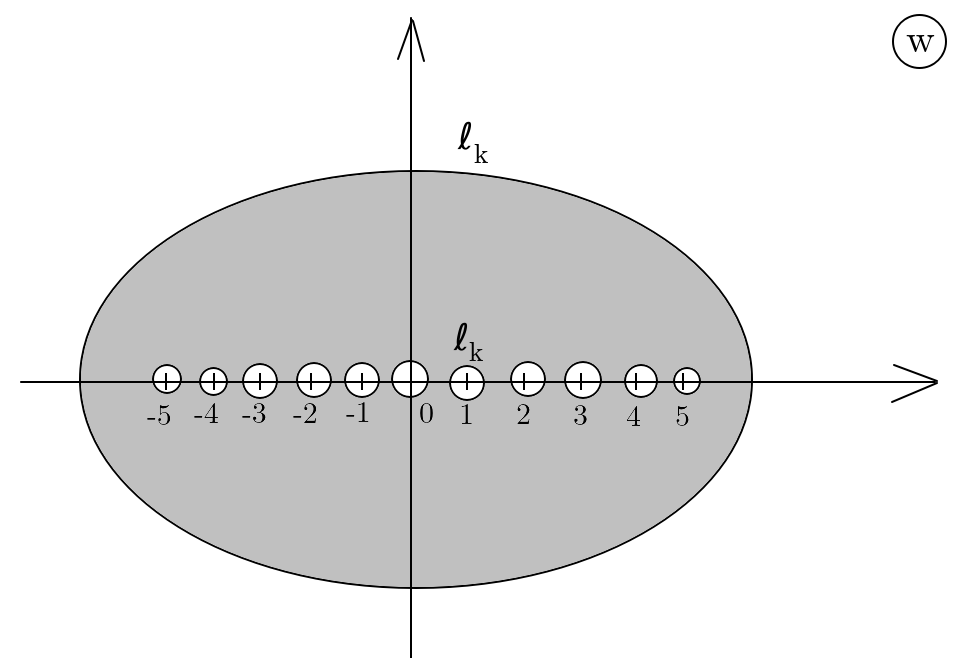
\includegraphics[width=0.6\textwidth]{lec32_4}
	\end{center}
	У подынтегральной функции особые точки находятся из уравнения:
	\[  \sin{\pi z} = 0 \implies z = k \in \Z, z = 0, \pm 1, \pm 2, \pm 3 , \pm 4 
	, \pm 5 \implies |z| < 5,\!1     \]
	Здесь 
	\[  I = \sum_{k=1}^{5} I_k       \]
	\[  I_k = \oint \limits_{l_k} \frac{dz}{\sin{\pi z}} = \oint \limits_{l_k} 
	\frac{\frac{z-z_k}{\sin{\pi z}}}{z-z_k} \ dz = \left[ \begin{gathered} f(z) = 
	\frac{z-z_k}{\sin{\pi z}} \underset{z \to z_k}{\rightarrow} \frac{1}{\pi 
	\cos{\pi z_k}} \\
	z_0 = z_k,\\ f(z) \ \text{аналитична в } \ D \subset l_k = \partial D_k 
	\end{gathered} \right] =          \]
	\[  = 2 \pi i f(z_k) = \frac{2i}{\cos{\pi z_k}}       \]
	\[   I = 2i \left( \frac{1}{\cos{0}} + \frac{2}{\cos{\pi}} + \frac{2}{\cos{2 
	\pi}} + \frac{2}{\cos{3 \pi}}  + \frac{2}{\cos{4 \pi}} + \frac{2}{\cos{5 
	\pi}}\right) = -2i.      \]
	\end{enumerate}
\end{examples}

\begin{corollary*}[теорема о среднем для аналитической ФКП]	
	Пусть $f(z)$ аналитична в круге $K_r = \left\lbrace z \  \big| \ |z-z_0| \le 
	r   \right\rbrace $. Тогда:
	\[   f(z_0) = \frac{1}{2 \pi i} \oint \limits_{|z-z_0| = r} 
	\frac{f(z)}{z-z_0} \ dz = \left[\begin{gathered} z-z_0 = r e^{i\phi} \\
	\phi \in [0,2\pi]  \\
	z = z_0 + r e^{i\phi} \\
	dz = r i e^{i\phi} d \phi
	\end{gathered} \right] = \frac{1}{2 \pi i} \int \limits_{0}^{2\pi} 
	\frac{f(z_0 +r e^{i\phi} ) i r e^{i\phi} d\phi}{r e^{i\phi}}  =     \]
	\begin{equation}
	\label{32:6}
	= \frac{1}{2 \pi } \int \limits_{0}^{2\pi} f(z_0 +r e^{i\phi} ) \ d \phi.
	\end{equation}
	\eqref{32:6} \--- среднее значение рассматриваемой аналитической $f(z)$  
	в круге $K_r$ с 
	центром $z_0$. В результате получаем, что среднее значение 
	равно $f(z_0)$ вне зависимости от используемого радиуса $r>0$.
\end{corollary*}
\begin{remark}
	Используя теорему о среднем, для аналитической ФКП можно пояснить, что 
	справедлива следующая теорема:
\end{remark}
\begin{theorem}[принцип максимума модуля аналитической ФКП]
	Если $f(z)$ аналитична в ограниченной области $D \subset \C$ и непрерывна на 
	$\overline{D}$, то $\exists M = \max \limits_{z\in D} |f(z)| \in \R^+$, 
	причем 
	$M$ достигается хотя бы в одной точке $z_0 \in \partial D$, т.~е. $M = 
	|f(z_0)|$.
\end{theorem}		
Из этой теоремы, в частности, получаем, что так как $\Re$ и $\Im$ аналитичной 
ФКП 
являются парой взаимносопряженных гармонических функций, удовлетворяющих 
уравнению Лапласа, то принцип максимума модуля для аналитических ФКП дает 
соответствующий принцип для гармонических действительных Ф2П.
	
\end{document}	
